
\documentclass{vgtc}                          % final (conference style)
%\documentclass[review]{vgtc}                 % review
%\documentclass[widereview]{vgtc}             % wide-spaced review
%\documentclass[preprint]{vgtc}               % preprint
%\documentclass[electronic]{vgtc}             % electronic version

%% Uncomment one of the lines above depending on where your paper is
%% in the conference process. ``review'' and ``widereview'' are for review
%% submission, ``preprint'' is for pre-publication, and the final version
%% doesn't use a specific qualifier. Further, ``electronic'' includes
%% hyperreferences for more convenient online viewing.

%% Please use one of the ``review'' options in combination with the
%% assigned online id (see below) ONLY if your paper uses a double blind
%% review process. Some conferences, like IEEE Vis and InfoVis, have NOT
%% in the past.

%% Figures should be in CMYK or Grey scale format, otherwise, colour 
%% shifting may occur during the printing process.

%% These three lines bring in essential packages: ``mathptmx'' for Type 1 
%% typefaces, ``graphicx'' for inclusion of EPS figures. and ``times''
%% for proper handling of the times font family.

\usepackage{mathptmx}
\usepackage{graphicx}
\usepackage{times}

%% We encourage the use of mathptmx for consistent usage of times font
%% throughout the proceedings. However, if you encounter conflicts
%% with other math-related packages, you may want to disable it.

%% If you are submitting a paper to a conference for review with a double
%% blind reviewing process, please replace the value ``0'' below with your
%% OnlineID. Otherwise, you may safely leave it at ``0''.
\onlineid{0}

%% declare the category of your paper, only shown in review mode
\vgtccategory{Research}

%% allow for this line if you want the electronic option to work properly
\vgtcinsertpkg

%% In preprint mode you may define your own headline.
%\preprinttext{To appear in an IEEE VGTC sponsored conference.}

%% Paper title.

\title{Monster Escape}

%% This is how authors are specified in the conference style

%% Author and Affiliation (single author).
%%\author{Roy G. Biv\thanks{e-mail: roy.g.biv@aol.com}}
%%\affiliation{\scriptsize Allied Widgets Research}

%% Author and Affiliation (multiple authors with single affiliations).
%%\author{Roy G. Biv\thanks{e-mail: roy.g.biv@aol.com} %
%%\and Ed Grimley\thanks{e-mail:ed.grimley@aol.com} %
%%\and Martha Stewart\thanks{e-mail:martha.stewart@marthastewart.com}}
%%\affiliation{\scriptsize Martha Stewart Enterprises \\ Microsoft Research}

%% Author and Affiliation (multiple authors with multiple affiliations)
\author{Evan Lin\\ %
    \parbox{1.4in}{\scriptsize  \centering\emph{Hunter College}}\\
    \scriptsize{evan.lin35@myhunter.cuny.edu}
\and Anik Singha\\ %
    \parbox{1.4in}{\scriptsize  \centering\emph{Hunter College}}\\
    \scriptsize{anik.singha68@myhunter.cuny.edu}
\and Josiel Perez\\ %
    \parbox{1.4in}{\scriptsize  \centering\emph{Hunter College}}\\
    \scriptsize{josiel.perez13@myhunter.cuny.edu}\\
\and Adrian Mysliwiec\\ %
    \parbox{1.4in}{\scriptsize  \centering\emph{Hunter College}}\\
    \scriptsize{adrian.mysliwiec13@myhunter.cuny.edu}
}

%% A teaser figure can be included as follows, but is not recommended since
%% the space is now taken up by a full width abstract.
%\teaser{
%  \includegraphics[width=1.5in]{sample.eps}
%  \caption{Lookit! Lookit!}
%}

%% Abstract section.
\abstract{Escaping reality is made possible by the rapid development of VR devices over the many years. To truly feel immersed, visuals, audio, haptics, and many more concepts are utilized to enhance the experiences in these worlds. It is essential to develop with a balance in mind which was the aim of our VR game. With a concentration in auditory and visual feedback, our group created a sense of eeriness and loneliness throughout the duration of the game.

Monster Escape is a multi-leveled exploration game aimed at escaping four various rooms. Beginning with the Office, followed by the Warehouse, Basement, then Backrooms, the player explores their environment to locate the next level. The levels increase in difficulty due to the challenges that are implemented. Progression is implemented in a way that is catered towards the player being able to explore each environment without a guide but not experience confusion. We opted to not have a guide in the game to limit the ability for the player to interact with any sort of living being to further reinforce a sense of loneliness in the game. All possible hope of being alone is eventually ruined with the introduction of a monster in the Warehouse. Balancing difficulty in a game with no guide can often be challenging because introducing new ideas must be done properly without making it too easy but also not making it too difficult. With this in mind, our group created an appropriate pace regarding the increase of difficulty.
} % end of abstract

%% Copyright space is enabled by default as required by guidelines.
%% It is disabled by the 'review' option or via the following command:
% \nocopyrightspace

%%%%%%%%%%%%%%%%%%%%%%%%%%%%%%%%%%%%%%%%%%%%%%%%%%%%%%%%%%%%%%%%
%%%%%%%%%%%%%%%%%%%%%% START OF THE PAPER %%%%%%%%%%%%%%%%%%%%%%
%%%%%%%%%%%%%%%%%%%%%%%%%%%%%%%%%%%%%%%%%%%%%%%%%%%%%%%%%%%%%%%%%

\begin{document}

%% The ``\maketitle'' command must be the first command after the
%% ``\begin{document}'' command. It prepares and prints the title block.

%% the only exception to this rule is the \firstsection command
\firstsection{Introduction}

\maketitle

%% \section{Introduction} 

Monster Escape was formulated with the intent to disorientate itself to constantly maintain an edge on the player. The initial challenge our group faced was not creating a limited experience that discourages the player but was not too easy to be traversed. Our main goal was to make an experience that perfectly balanced how challenging it was and how engaging it was for players. We were aware of the fine line we had to walk: we didn't want to make the experience too limited and dull, which could turn players off, but we also didn't want it to be too easy, which would take away the fun of exploring and finding new things.

The game takes players on a journey through many levels, with each one being trickier and scarier than the last. Our virtual journey starts in the harmless Office and goes down into the Warehouse, the mysterious Basement, and the scary Backrooms. Each stop will test your resolve to the fullest. The levels of difficulty in the game are carefully thought out so that players can get through these confusing areas without needing a hand to hold, but this doesn't let confusion set in.

An interesting part of our VR experience is that there is no one there to guide us. This is done on purpose to add to the intense feeling of loneliness and unease that permeates the game. But, just like some people find comfort in being alone, our players quickly learn that their solitude isn't permanent. As they go deeper into the Warehouse, a sneaky monster appears and breaks the illusion that they are truly alone.

It was hard to find the right balance of difficulty in a world where you weren't being led anywhere. We knew that adding new ideas and challenges had to be done carefully, finding that tricky middle ground where the experience is neither too easy nor too hard to handle. Because of this, our hardworking team carefully set the right rate of difficulty increase to make sure that the excitement of exploration and the challenge of discovery were always in perfect balance.

In this review of Monster Escape, we go deep into the heart of a virtual reality journey that breaks the rules, creating a story of disorientation and tension while pushing the player to face their fears and figure out the mysteries that lie within.



\section{Exposition}

In recent years, the realm of virtual reality has undergone a transformative evolution, ushering in a new era of immersive experiences that challenge the boundaries of the physical and digital worlds. It is within this landscape of technological innovation and limitless possibilities that "Monster Escape" was conceived, not merely as a game but as a journey that plunges players into the heart of virtual realms.

The core principle guiding the development of "Monster Escape" was immersion. We sought to create a virtual world that not only captivates the senses but submerges players in an alternate reality, where every visual, auditory, and sensory detail is meticulously crafted to blur the lines between the real and the virtual. This pursuit of immersion became the foundation upon which our game was built.

The premise of "Monster Escape" is simple yet enthralling: players are tasked with escaping a series of levels, each one shrouded in mystery and riddled with challenges. It is in the pursuit of escape that we leverage various elements to intensify the immersive experience. Interactivity plays a central role, allowing players to engage with their surroundings and manipulate the environment, bridging the gap between observer and participant.

Sound design, lighting, and ambience were carefully orchestrated to envelop players in an atmosphere that feels palpably real. The echo of footsteps in empty corridors, the play of light and shadows on the walls, and the faint hum of machinery in the distance—all of these elements were meticulously crafted to foster an environment that is both captivating and unsettling. The aim was not just to engage the eyes and ears but to make players feel the world around them, immersing them in an experience that goes beyond mere visuals.

While immersion is a central theme, "Monster Escape" does not shy away from challenging players. Navigating the levels can be a formidable task, requiring critical thinking, problem-solving, and sheer determination. Each level is carefully designed to present a unique set of challenges, ensuring that players are consistently engaged and compelled to overcome the hurdles in their path.

One of our primary sources of inspiration was the concept of "The Backrooms." In this intriguing concept, an unsuspecting individual finds themselves inexplicably dropped into an endless iteration of an aging office space. What makes "The Backrooms" concept so compelling is the notion of "liminal space"—spaces that are neither here nor there, abandoned yet hauntingly familiar. It's as if someone had once lived in these environments, and their lingering presence, although absent, evokes an eerie and surreal feeling.

In "Monster Escape," we aimed to capture the essence of "liminal space" and infuse it into each level, making players question the reality of their surroundings and heightening the overall sense of eeriness. The very architecture of our game world is designed to invoke this unsettling and uncanny feeling, mirroring the very heart of "The Backrooms" concept.

As we delve deeper into the design and experience of "Monster Escape," we will explore the intricate tapestry of immersion, interactivity, and challenges that make our virtual journey an unforgettable adventure. It is a world where reality blurs with the virtual, where players must escape not just from levels but from the very confines of their own perception.

\section{The Office}

\begin{figure}[htb]
  \centering
  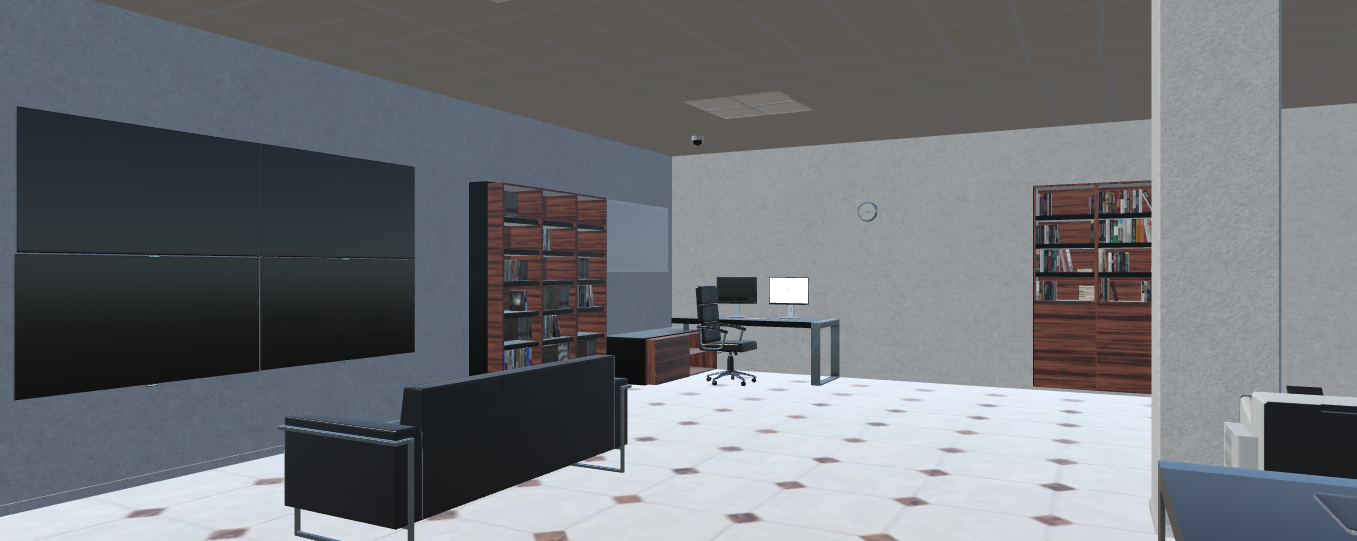
\includegraphics[width=1.5in]{The Office.png}
  \caption{The office spawn room}
\end{figure}

The office level presents the player with a hauntingly lonely office setting that seems familiar but is strangely quiet. The aesthetic effectively conveys the spirit of a typical setting, but the sense of mystery is enhanced by the desolation. Finding hidden collectibles—relics from the past life that used to occupy this space—is the main objective in this landscape of abandoned desks and chairs. Along with gathering, there's also the quest to find the elusive elevator. This elevator is a doorway to the warehouse world, a haven from the quiet emptiness of the office. To increase the immersion aspect, the soundscape may play gentle hums from malfunctioning machinery or far-off phone ringing throughout this level. Despite the large workspace, the design keeps players focused and interested without making them feel overly disoriented. In a final act of kindness, the challenges gradually lessen as players get closer to the finish, enabling them to move to the warehouse and see what's coming next.

\section{The Warehouse}

\begin{figure}[htb]
  \centering
  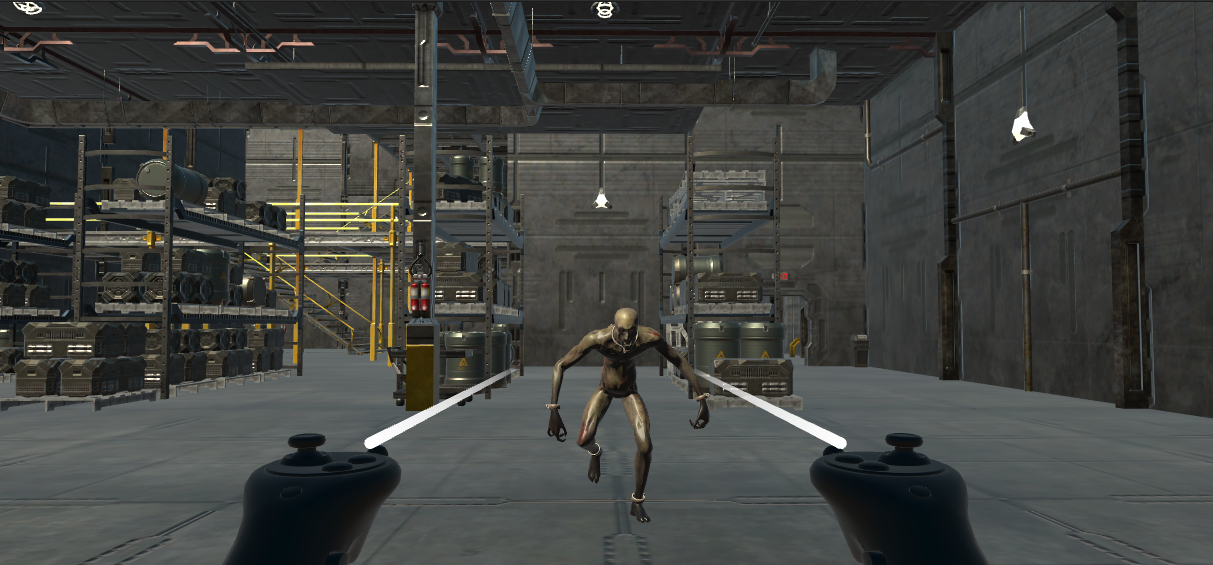
\includegraphics[width=1.5in]{monster.png}
  \caption{The monster}
\end{figure}

The warehouse level is the first encounter the player has with the monster. The warehouse seems almost alien, with the materials the floors and walls are made of, as if they're too futuristic for this current time. This level heavily focuses on the horror aspect, as you are being chased by the monster with no current means to fight back, so the only goal is fight back and survive. The monster can hurt the player, driving home the fact that the player must escape. The level also focuses on immersion, through things like sounds (ambience and hearbeats). The level is also big but not huge enough for the player to get lost in. The monster only attacks whenever the player is close enough, and will track the player down no matter where they are due to a nav mesh. At the end, in order to make things more fair, the monster is stopped from entering a certain part, so the player can progress to the next level safely.

\section{The Basement}

\begin{figure}[htb]
  \centering
  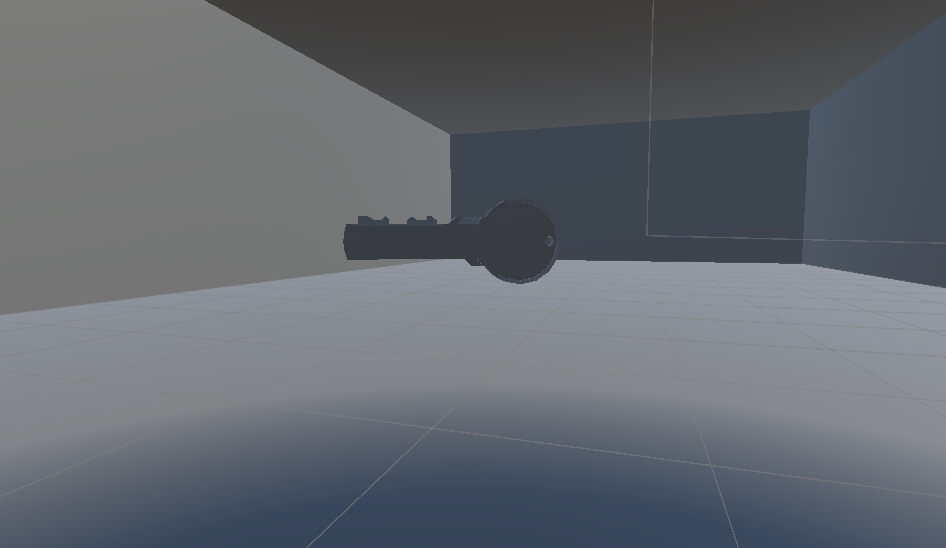
\includegraphics[width=1.5in]{key.png}
  \caption{Collectible key}
\end{figure}

The basement level is meant to put the player back into a familiar yet mysterious environment. The warehouse had a type of sci-fi aesthetic to it, but the basement will be an environment that most people have probably seen in real life. The level was designed using probuilder and is meant to have an open feel. There are no doors anywhere and every room is connected to each other. There will be a bit of linear exploration in this level. The player is meant to find a certain number of keys, which when collected will allow them to visit the next level, which is the maze. A key can be collected by coming within a certain distance of it. While we’ve already created the layout of the level, we are yet to add any textures. We hope to find a good texture pack which will help us achieve the feeling we are going for with this level. We hope to create a very interesting visual and auditory experience in this level by the end stage of the project. 

\section{The Maze}

\begin{figure}[htb]
  \centering
  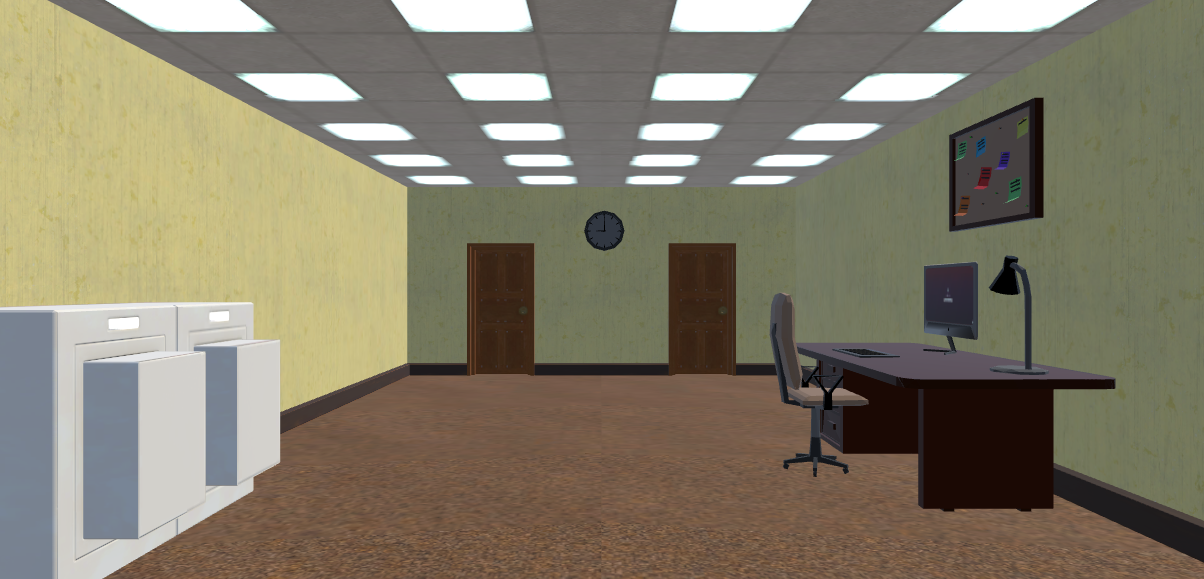
\includegraphics[width=1.5in]{The Maze.png}
  \caption{Starting room of the maze}
\end{figure}

The purpose of the maze level was to create an environment that was seemingly normal but also incredibly eerie and mysterious. We wanted to invoke feelings similar to that of ones created by the uncanny valley. Our initial inspiration was taken from “The Backrooms”, which is a popular internet story about a never ending liminal space. Similar to past levels, the goal is to obtain a certain number of collectibles that will then unlock a door to the final boss fight. We started off the development cycle by creating the environment, which is the most important aspect of this level. We created many different rooms and then connected them to one another in such a way that it was very easy to get lost. Eventually we realized that this level could potentially become boring to players, since most of the rooms they visited were copies of one another. Due to this, we decided to add a bit more life to the rooms by adding different office props. Luckily, even after adding props, the level still maintained the same level of eeriness. In order to add realism, we added sound effects for the door opening and closing. Eventually we’d also like to add some interactivity, such as creating books with different notes which players can find and read. 

\section{Developing the Office}
The design of the Office level necessitated meticulous planning and implementation to achieve a seamless integration of both the environmental aspects and the desired player experience. The design process adopted a narrative-driven approach, similar to that of Monster Escape. An essential emphasis was placed on building a logical and captivating design, connecting chambers, and, of course, generating a compelling and immersive starting point for the player. The layout design step entailed the conversion of generic room spaces into realistic office environments, requiring meticulous attention to detail. This was necessary not just to achieve the desired aesthetic, but also to guarantee that the theme conveys a narrative element. To achieve authenticity, it was necessary to decorate these spaces with a diverse array of meticulously positioned everyday office artifacts. Moreover, the inclusion of interactive features such as door answers serves to heighten the feeling of authenticity and foster active participation, contributing to a combination of anticipation and discovery within interconnected areas. The primary objective in building the Office level was to provide players with strong incentives to completely investigate every area of The Office. To further support this objective, scattered keys were incorporated as an additional element. The keys are strategically positioned in various locations, and players are encouraged to locate them by thoroughly exploring the environment in order to advance. Acquiring keys advances the player's progress towards opening the ultimate entrance to the warehouse, introducing a hard element to the game and providing a sense of achievement. In summary, the development of The Office level required careful strategizing to create an engaging gameplay experience through a combination of contextual storytelling and interactive gameplay. This allowed players to navigate through both the empty Office and the more difficult Warehouse sections. 

\section{Debugging the Office}
The refinement of the game involved a constant process of discovering and resolving technological issues. Ensuring the smooth operation of scripts across different components in the game proved to be one of the most intricate aspects of this procedure. A significant amount of time and effort was dedicated to thoroughly validating the proper functionality of each script and its integration with the related object in the game's environment. Another notable obstacle entailed the execution of functional collision mechanics. It was crucial to preserve the integrity of the entire game world in order to avoid things from falling through the floor. Testing was extensively conducted to ensure that the game's collision properties were applied accurately to the objects, resulting in a functional and interactive physics system. Moreover, incorporating the random office items into the room decor had its own challenges. The first selection of assets lacked compatibility with the game's "grab" interaction, which forced a complete overhaul of the room's design using new components that were totally compatible. The ultimate objective was to design a seamless and captivating experience for players, ensuring that every aspect of the game contributed to the desired atmosphere and objectives within the game's world. Successfully navigating and conquering these obstacles demonstrates the dedication, perseverance, and expertise necessary for creating a game that is both refined and captivating. 

\section{Developing the Warehouse}
The development of the warehouse level in Monster Escape involved expanding upon the initial warehouse demo. In this latest version, we have enhanced the terror element by introducing a concrete consequence of being unable to leave, which is represented by a Health Points (HP) system. In addition, to provide players with a clear aim and a concrete goal, we have incorporated an objective within the level. This objective requires the player to activate three switches in order to reactivate the exit to the level. To enhance the level's immersion, interaction and sound played a significant role. We have incorporated manipulable items in the form of switches, as well as dynamic doors that respond accordingly. In terms of sound, the player's heartbeat responds to the monster's presence, providing information about both the distance and the level of risk posed by the creature. In addition, levers produce an audible signal at full activation to indicate to the player the completion of this aim. The user interfaces played a crucial role in our design, as we considered the necessity of displaying the player's health points and the progress of the objectives. Due to the virtual reality nature of this project, we encountered several challenges in devising a method to visualize these concepts. We developed a user interface (UI) that is connected to the player's wrist. This UI interacts with the gaze interactor and only appears when the player's palm is facing towards them. In addition, a pause menu and a game over menu were implemented as supplementary features to enhance the user experience.

\section{Debugging the Warehouse}
With the introduction of this version of the warehouse, numerous problems emerged. For example, a task as basic as manipulating items in virtual reality posed a significant challenge. Subsequently, I had to address the problem of obtaining the levers. Initially, I adopted the concept of hands that were impacted by collision. However, owing to time constraints, I had to abandon that notion and instead focus on simpler hands. While I was engaged in manipulating the levers, I encountered peculiar glitches. Curiously, the levers functioned exclusively along the z-axis, but experienced considerable damage when the rotation was adjusted to the x-axis. In addition, the process of building the user interface presented its own set of difficulties. The pause menu initially experienced a problem of being synchronized with the camera's focus. I have to correct it in order to ensure its immobility upon activation. Subsequently, I lacked the opportunity to rectify this matter, nevertheless, the user interface experiences a decrease in responsiveness when the menus are enabled. Regrettably, I was unable to address this issue due to time limitations.

\section{Developing the Basement}
During the development of Monster Escape, numerous concepts were conceived, executed, and possibly discarded. An ongoing topic of discussion in the early stages was the concept of fluidity and how the many levels should interact, particularly from a narrative perspective. Given the project's inspiration from the Backrooms concept, it was finally determined to prioritize a design that lacks fluidity while still preserving the mechanics. The Ghoul was conceived in the Warehouse as part of the Office to Warehouse to Basement to Maze concept, and it pursues the player as they progress through the lower levels. Zooming in on the Basement scene, one of the more demanding components of this scene was the arrangement of the room. It is crucial to achieve a harmonious equilibrium between exploration and avoiding both desolation and excessive size. After completing the initial design, the following step was to incorporate a specific goal for the player. By implementing diverse C-sharp scripts, collectibles were incorporated to enable the player to advance to the Maze once a specific number of them had been gathered. The next task on the agenda involved installing different light fixtures in the Basement. The rationale behind this is the presence of minimal illumination, except from the flashlight which will be addressed subsequently. An amalgamation of animation, C-sharp programming, and audio sources creates an interactive and immersive experience, enabling the user to activate the room's light source by flipping a small switch. Expanding on the concept of light sources, a flashlight was developed to allow the player to easily access and operate the buttons for turning on and off. This enables the room's design to replicate the ambiance of a frigid, dim, and isolated space. The ultimate element of this scene involved advocating for a design that is of a moderate size, neither excessively large nor disappointing, and possesses excellent movement for the Ghoul. The utilization of diverse textures and elements evokes a disquieting atmosphere of alone for the player, while simultaneously suggesting the possibility of someone's presence.

\section{Debugging the Basement}
At each stage, there were issues that required attention and troubleshooting. Conducting collision experiments was crucial since it allowed us evaluating the scenario with both keyboard/mouse and the VR headset, as the interactions differed. Several experiments have demonstrated that incorporating a collider into both the camera and walls enables Unity to accurately detect two solid objects and avoid any form of overlapping. Eliminating defects entirely is an unattainable goal in coding. Therefore, during the creation of the objective and collectible scripts, numerous errors were detected during runtime when the script failed to activate or delete the associated game object correctly. Research shown that by correctly assigning the scripts to the appropriate game objects and setting their associated values in the components tab, it was possible to trigger events such as the appearance of the next level screen when the collectible goal was achieved. Ensuring a seamless and efficient interaction between the hands and any objects that can be manipulated. An instance where debugging was required arose when troubleshooting was needed to enable the functionality of the light switch on the virtual reality (VR) headset, which was only operational while using a keyboard and mouse (KBM). By doing tests on different colliders and modifying the Lightswitch script, we successfully resolved the problem that allowed the hand to enter the lightswitch zone and toggle the light. In the end, the scene's final result was refined and seamless to ensure an optimal user experience.

\section{Developing the Maze}
The complexity of the maze level was significantly increased following the submission of the midterm demo. Additional rooms were incorporated, accompanied by a subterranean labyrinth. We were unequivocally determined to create an underground labyrinth that would serve as a setting for the player to be relentlessly pursued by the monster, necessitating their survival skills. Nevertheless, we were uncertain about the specific purpose we intended the other rooms to fulfill. The containers lacked contents and had an exceptionally dull taste. Ultimately, we conceived the notion of locating collectibles in order to gain access to a door that would lead us to the subterranean area. In order to increase the level of difficulty in finding the keys, we made the deliberate choice to furnish the chambers with numerous objects. Every room possessed a distinct ambiance and arrangement. The rooms are furnished with various settings, including a garage, a dining hall, a medieval library, a classroom, and a morgue. The settings in our game, Monster Escape, may appear arbitrary, but this was intentional as the game is designed to simulate a dream-like experience. Subsequently, luminescent keys were inserted into every door, amounting to a total of 9 rooms, with varying sizes. In prior levels, keys were also present and had to be collected, but their collection was determined by proximity. The key in my level can only be acquired by physically seizing it. Upon acquisition, a message would promptly appear on the display, indicating the successful collection of the key. The remaining quantity of keys would also be displayed on the panel affixed to your left wrist. An NPC was included to communicate the aim of the level to the player. He possesses a speech bubble positioned over his head that continuously displays various texts in a repetitive manner. Additionally, he exhibits animation as evidenced by his subtle respiration and gradual movements. Despite our efforts, we were unable to find an appropriate voice for him and we were unwilling to ourselves provide the voice. In relation to sound, we additionally incorporated the inclusion of footfall to enhance the game's sense of immersion. The purpose of the maze is to evoke a sense of emptiness. The inclusion of footsteps and the auditory cues of the doors opening and closing contributed to a disquieting atmosphere, evoking a sense of unease and uncertainty.

\section{Debugging the Maze}
Certain technological components of the maze level posed significant challenges in terms of coding and debugging. Firstly, I will address the less challenging aspects. It took approximately 30 minutes to compose the script for generating footstep noises. Due to our prior familiarity with audio from our work on the opening and closing door noises, the process of creating the steps was not overly challenging. The footstep sound would be triggered if the player had covered a specific distance and a specific amount of time had elapsed. Identifying the optimal time duration for playing the footsteps in order to provide a natural sound proved to be challenging. Transitioning from sound, this level extensively utilized texts and canvases. Two instances comprise the "key collected!" text, which manifests each time the user acquires a key, and the text bubble positioned above the non-playable character (NPC) who assigns the player the objective. Implementing the feature for the "key collected" proved to be a challenging task. We aimed to position the key above the gathered key without intersecting with any other objects, however we were unable to resolve this issue. We employed a mathematical algorithm and the LookAt function to ascertain the precise positioning of the text. The text may intersect with other items depending on the direction in which you gaze when retrieving the key. The task of generating the text bubble positioned above the non-playable character (NPC) proved to be highly challenging. We dedicated a significant amount of time to implement the functionality of displaying the subsequent text through user input, specifically by means of a button hit. We are uncertain of the reason, but it just did not function. Ultimately, we resolved to transition to the subsequent conversation once a specific duration had elapsed. Upon completion of the NPC's task, it would promptly recommence from the initial stage. We have also developed additional scripts that are associated with the keys. We need a script that encompassed a set of instructions for handling the event of key collection, as well as other scripts pertaining to key-related functions. A script was implemented to determine the locked status of a door based on the presence of all collected keys. Writing the scripts was often straightforward. Additionally, there was the task of generating and managing the ghoul's behavior. A pre-existing script was available to govern the behavior of the monster in a previous level, but we had to make some adjustments to adapt it for use in the maze level.

\section{Links}
\subsection* {Github Repository}
https://github.com/evanlin-dev/VR-Class-Project
\subsection*{Youtube Demo}
https://www.youtube.com/watch?v=D1E4Bvuo52g
\end{document}